
\chapter{Mining}

Het deelnemen aan de proof-of-work loterij om de kans te krijgen het bitcoin grootboek aan te passen, staat beter bekend als het \textit{minen} van bitcoins. Hieruit volgt hoe dit in zijn werk gaat:

\begin{enumerate}
    \item Iedereen die wil deelnemen, sluit zich aan bij het bitcoinnetwerk door hun computer aan te zetten, de juiste bitcoin-software te draaien en te luisteren naar anderen die hun transacties aankondigen.
    \item Alice kondigt haar voornemen aan om wat munten naar Bob te sturen. De computers op het netwerk \textquotedbl{}roddelen\textquotedbl{} met elkaar om deze transactie naar iedereen op het netwerk te verspreiden.
    \item Alle computers die willen deelnemen aan de loterij starten met het \textit{hashen} van de transacties waar ze over hebben gehoord door willekeurige \textit{nonces} toe te voegen aan de transactielijst en de sha256 \textit{hash}-functie uit te voeren.
    \item Gemiddeld elke tien minuten vindt een computer een hash afgeleid van de transacties die lager is dan het huidige doelnummer en wint daarmee de loterij.
    \item Deze computer maakt zijn winnende getal bekend, evenals de invoer (transacties en nonce) die ze hebben gebruikt om het winnende lot te produceren. Het kan uren gekost hebben om dat te vinden, of een paar minuten. Deze informatie bij elkaar (transacties, nonce en de hash van het proof-of-work) wordt een \textit{blok} genoemd.
    \item Alle andere deelnemers valideren het blok door te controleren of de transacties in het blok, in combinatie met de nonce, daadwerkelijk resulteren in de gedeelde hash. Ze kijken ook of de hash inderdaad lager is dan het doelnummer, of het blok geen ongeldige transacties bevat en of de geschiedenis in het blok niet in tegenspraak is met eerdere blokken.
    \item Iedereen schrijft het blok in zijn kopie van het grootboek en voegt het toe aan de bestaande ketting van blokken, bekend als een \textit{blockchain}.
\end{enumerate}

Dat is het in een notendop. We hebben ons eerste blok geproduceerd en mogen onze eerste transacties aan onze grootboeken toevoegen.

Je hebt mogelijk in de media de bewering gehoord die vaak wordt herhaald: bitcoin mining zou inhouden dat je complexe vergelijkingen oplost. Maar nu zal je begrijpen dat dit een misvatting is. Bij bitcoin mining gaat het er niet om dat je vergelijkingen oplost, maar dat je voortdurend een grote virtuele dobbelsteen werpt om een hash te genereren die onder een specifiek doenummer valt. Eigenlijk is het gewoon een kansspel, waarbij de deelnemers verplicht zijn om een bepaalde hoeveelheid elektriciteit te gebruiken.

\section{Hoe worden nieuwe bitcoins gemaakt?}

Tot dusver hebben we het gehad over hoe Alice \$2 naar Bob kan overmaken. Maar vanaf nu zullen we niet meer spreken over dollars, aangezien bitcoin deze valuta niet kent. Waar we wel over beschikken, zijn bitcoins zelf: digitale eenheden die waarde vertegenwoordigen binnen het bitcoinnetwerk.

Om bij ons voorbeeld te blijven, kunnen we zeggen dat Alice 2 bitcoins naar Bob stuurt door aan te kondigen dat ze haar munten, die op haar \textquotedbl{}rekening\textquotedbl{} staan, naar die van Bob overzet. Vervolgens wint iemand de proof-of-work loterij, en wordt haar aangekondigde transactie toegevoegd aan het grootboek.

Maar waar kwamen die 2 bitcoins van Alice oorspronkelijk vandaan? Hoe ging bitcoin van start en hoe verwierf iemand ooit munten voordat er marktplaatsen waren om ze te kopen met traditionele fiatvaluta zoals dollars of euro’s?

Toen Satoshi bitcoin bedacht, had hij ervoor kunnen kiezen een database op te zetten waarin alle 21 miljoen munten aan hem werden toegekend, om vervolgens iedereen te vragen deze van hem te kopen. Echter, er zou weinig reden zijn voor anderen om waarde toe te wijzen aan een systeem waarin één persoon alle waarde bezit. Hij had ook een register kunnen creëren waar mensen zich konden aanmelden met een e-mailadres om kans te maken op een paar munten. Zo'n registratiesysteem zou echter gevoelig zijn voor een zogenaamde \textit{Sybil-aanval}, aangezien het praktisch kosteloos is om miljoenen e-mailadressen te genereren.\footnote{Een Sybil-aanval is een aanval waarin een deelnemer aan een bepaald netwerk een groot aantal pseudonieme addressen aanmaakt om een grote hoeveelheid invloed in het netwerk te vergaren; vernoemd naar Sybil, een boek over een vrouw met een dissociatieve identiteitsstoornis}

Uiteindelijk besloot Satoshi dat de nieuwe munten gegenereerd zouden worden door het proces van minen, ofwel het deelnemen aan een zogenaamde proof-of-work loterij om het recht op schrijven in het grootboek te bemachtigen. Als je veel energie verbruikt en het winnende nummer van het volgende geldige blok vindt, krijg je het recht om de transacties te registreren die je kent in het grootboek. Bovendien mag je een speciale transactie aan het blok toevoegen, wat we een \textit{coinbase}-transactie noemen. Die transactie houdt in \textquotedbl{}dat 12,5 bitcoin werden gemaakt en toegekend aan Marie de Miner om haar te compenseren voor de energie die gebruikt werd om het blok te vinden.\textquotedbl{}

Dit is hoe nieuwe bitcoins \textquotedbl{}gemaakt\textquotedbl{} worden. Met dit proces is iedereen ter wereld in staat om hun eigen munten te vergaren zonder tussenkomst van een centrale autoriteit én zonder hun identiteit bekend te moeten maken. De enige vereiste is dat ze genoeg willen betalen voor de elektriciteit die nodig is om mee te doen met de loterij. Dit maakt bitcoin’s uitgifte resistent tegen \textit{sybil}-aanvallen. Wie munten wil, zal energie moeten verbruiken en iets moeten betalen om ze te maken.

\section{De beloning per blok}
De persoon die de loterij wint, mag zichzelf enkele vers gemaakte munten toekennen. Maar waarom is de beloning 12,5 bitcoins en niet 1000? Hoe kan het dat niemand de boel kan bedriegen en zomaar een willekeurig bedrag in de wacht kan slepen?

Bitcoin is een systeem gebaseerd op gedistribueerde consensus. Dit betekent dat elke deelnemer het eens moet zijn over wat geldig en wat ongeldig is. Dit wordt bereikt door software te gebruiken die bepaalde, algemeen aanvaarde regels afdwingt. Deze regels zijn bekend als de consensusregels van bitcoin. Als een miner een nieuw blok vindt, wordt dit tegen deze consensusregels aangehouden. Indien het blok overeenkomt met de regels, wordt het door alle deelnemers in hun grootboek genoteerd en als waarheid geaccepteerd. Als dit niet het geval is, wordt het blok afgekeurd.

Hoewel de volledige lijst met consensusregels behoorlijk ingewikkeld kan zijn, kunnen we de meest belangrijke hieronder voor je opsommen:

\begin{itemize}
    \item Een geldig blok mag een bepaalde hoeveelheid nieuwe munten aan het netwerk toevoegen, mits het zich houdt aan de regels van het uitgifteschema dat is vastgelegd in de software.
    \item Transacties dienen geldige handtekeningen te bevatten die bevestigen dat de eigenaar daadwerkelijk akkoord is gegaan met de verzending.
    \item Transacties waarbij men probeert reeds uitgegeven munten opnieuw uit te geven, zijn onder geen enkele omstandigheid mogelijk.
    \item De hoeveelheid data in het blok mag een specifieke limiet niet overschrijden.
    \item De proof-of-work hash van het blok moet kleiner zijn dan het huidige doelnummer. Dit vormt een onweerlegbaar bewijs dat er een bepaalde hoeveelheid stroom is verbruikt om dit blok te genereren.
\end{itemize}

Als Marie een blok vindt en besluit om zichzelf een extraatje te geven, zullen de computers van de andere deelnemers dit blok afwijzen en als ongeldig beschouwen. Dit komt omdat de bitcoin-software die iedereen gebruikt, een stukje code bevat dat zegt: ``de huidige beloning voor een blok is exact 12,5 bitcoins. Als je een blok tegenkomt waarin iemand meer dan dit bedrag toekent, wijs het dan af.''

Wanneer Marie probeert te frauderen door een ongeldig blok aan te maken, zal dit blok in niemands grootboek terechtkomen en zal ze alleen maar een hoop elektriciteit hebben verspild om een vervalsing te creëren die niemand wil hebben. Dit geeft bitcoin een \textit{onvervalsbare kostbaarheid}, een term die werd geïntroduceerd door Nick Szabo in zijn esssay \textquotedbl{}Shelling Out\textquotedbl{}. Het is gemakkelijk te begrijpen dat geld dat makkelijk te vervalsen is, nooit echt nuttig kan zijn als betaalmiddel. Het is onmogelijk om een bitcoin te vervalsen aangezien de authenticiteit van elke munt kan worden nagegaan met een eenvoudige wiskundige test.

Satoshi ontsloot het eerste genesisblok, waarmee de allereerste bitcoins gecreëerd werden. De code is open source, dus iedereen kan erin duiken om te controleren of alles in orde is. Maar zelfs Satoshi moest miljarden berekeningen verrichten en meedingen in de proof-of-work loterij om de eerste blokken te ontdekken. Er was geen manier waarop hij een vervalsing kon creëren door te liegen over de energie die nodig was om een winnende oplossing te vinden. En dat ondanks dat hij de bedenker was van het systeem.

Iedereen die zich daarna bij het netwerk aansloot kon controleren dat zijn gevonden oplossingen voldeden aan de vereisten. Door ze naast het initiële doelnummer en transactiedata te leggen, blijkt overduidelijk dat een bepaalde hoeveelheid energie gebruikt werd om een statistisch zeldzaam doelnummer te vinden. Stel je voor dat het mogelijk is om met diezelfde precisie en regelmaat te controleren hoe fiatvaluta in het traditionele bankensysteem tot stand komt.

\section{De halvering}
Het mijnproces genereert nieuwe bitcoins. Maar Satoshi wilde een systeem creëren waarin de valuta niet gedevalueerd kon worden. Hij was er geen voorstander van dat de geldhoeveelheid oneindig zou blijven groeien. In plaats daarvan ontwikkelde hij een uitgifteschema dat snel op gang kwam en geleidelijk afnam, totdat er uiteindelijk geen nieuwe munten meer geproduceerd zouden worden.

In het begin was de beloning voor een blok 50 bitcoin en dat is hoeveel Satoshi ontving voor zijn allereerste ontgonnen blok. Net zozeer kregen alle andere deelnemers die zich aansloten bij het netwerk in de begindagen voor elke gevonden blok 50 bitcoin.

De bitcoin-software dwingt iedere vier jaar een halvering van de blokbeloning af. De periode is gebaseerd op het aantal blokken in plaats van een bepaalde periode van tijd, maar omdat blokken ongeveer elke tien minuten worden geproduceerd, maakt dit in werkelijkheid weinig verschil. In 2008 was de blokbeloning 50 BTC, in 2012 was het 25 BTC, in 2016 12,5. Vandaag, op 8 juni 2019, zijn al 579.856 blokken ontgonnen sinds het begin van bitcoin en is de beloning 12,5 BTC per blok.

Binnen de volgende 50.144 blokken, rond mei 2020, zal de beloning verminderd worden tot 6,25 BTC per blok. De jaarlijkse toename van het aanbod wordt dan ongeveer 1,8\%. Na nog eens 12 jaar, 3 halveringen later, zullen 99\% van alle bitcoins in circulatie zijn en krijgen miners nog minder dan 1 bitcoin per gevonden blok. Je kan de voortgang van de halveringen volgen op \href{https://bitcoinblockhalf.com}{https://bitcoinblockhalf.com}.

\begin{figure}[h]
    \centering
    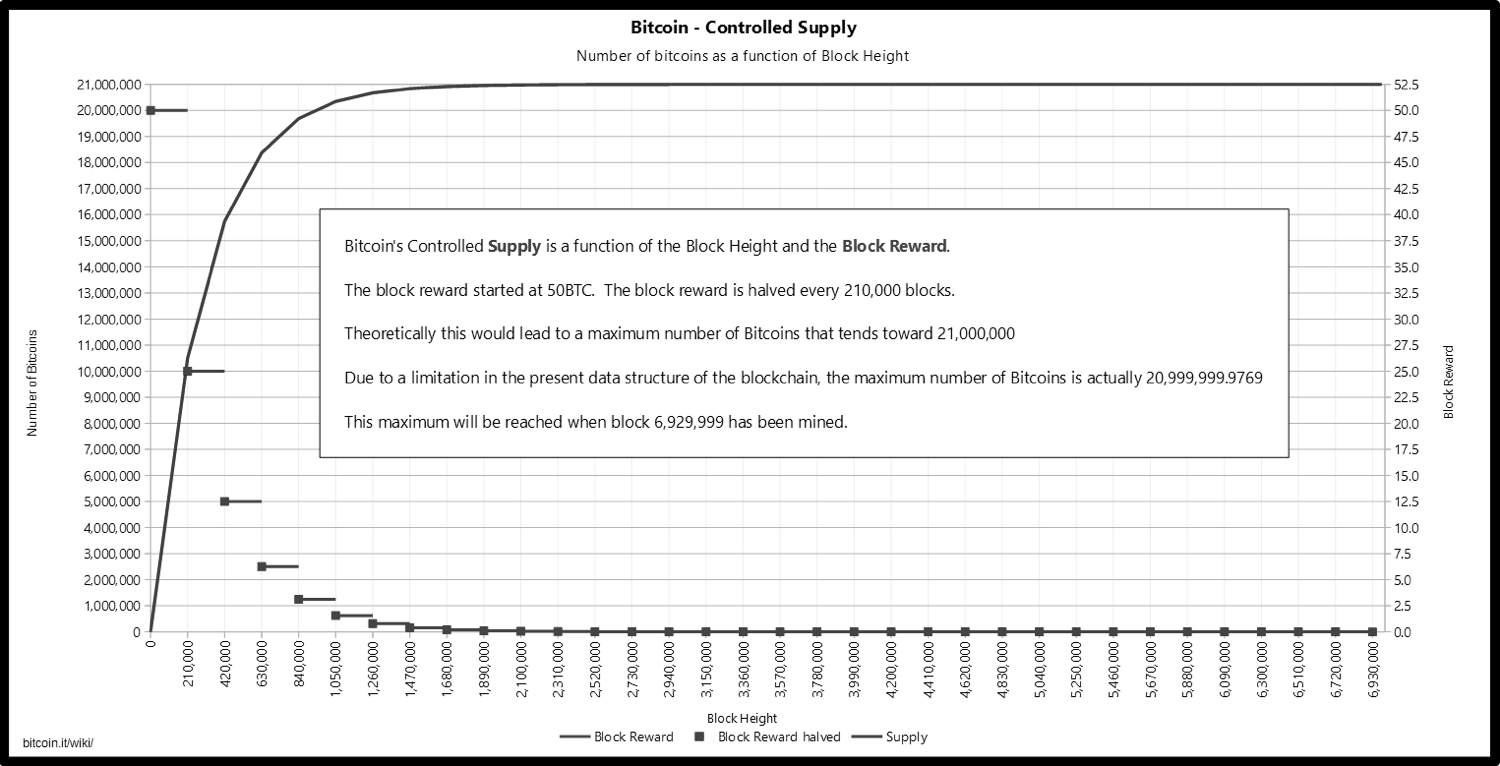
\includegraphics[width=\textwidth]{images/fig6.png}
    \caption{\footnotesize{\textit{Het gecontroleerde monetaire tijdschema van bitcoin kan door iedereen worden bevestigd.}}}
    \label{fig6}
\end{figure}

Uiteindelijk zal rond het jaar 2140 de beloning per blok volledig vervallen en zullen de miners enkel nog de transactiekosten van de gebruikers als vergoeding voor hun werk ontvangen.

De blokbeloningen en het uitgifteschema in het algemeen zijn verankerd in de bitcoin-software. Deze software is, zoals eerder vermeld, volledig open source. Iedereen kan deze dus controleren en valideren. Een blok dat niet aan de regels voldoet, zal door niemand met dezelfde software worden geaccepteerd.

\section{Beheersen van de uitgifte en het blokinterval}

Het minen van bitcoin vereist computers en elektriciteit. Dus hoe meer rekenkracht en elektriciteit je ter beschikking hebt, hoe groter de kans dat je de winnende combinatie kraakt Laten we zeggen dat het netwerk bestaat uit 100 computers met dezelfde rekenkracht en jij er 10 van bezit. Dit betekent dat jij in ongeveer 10\% van de gevallen de winnende oplossing zult vinden. Echter, het delven van bitcoins is een proces dat berust op geluk en toeval. Het kan dus theoretisch gezien voorkomen dat er uren of zelfs dagen voorbijgaan zonder dat je de winnende combinatie kunt kraken.

In het voorgaande deel hebben we uitgelegd dat miners zichzelf niet zomaar een willekeurige blokbeloning kunnen toekennen. Deze zou door andere \textit{nodes} worden afgewezen. Maar wat gebeurt er als zij veel energie gebruiken om het miningproces te versnellen en op die manier meer bitcoins te bemachtigen? Dat zou tegenstrijdig zijn met de ontwerpdoelstelling van bitcoin, waarbij het uitgifteschema van tevoren vast moet liggen.

Laten we nogmaals terugkeren naar het eerder aangehaalde voorbeeld: we hebben 1000 mogelijke hashes en ons doelcijfer is 100. In ongeveer 10\% van de gevallen zullen we een getal vinden dat kleiner is dan 100, en daarmee een geldig blok ontdekken.

Laten we aannemen dat het 1 seconde duurt om elke hash te berekenen. Als we elke seconde "onze dobbelsteen werpen" door de huidige transacties en onze willekeurige \textit{nonce} te hashen, vinden we in 10\% van de pogingen een getal dat kleiner is dan het doelnummer. We verwachten daarom dat we gemiddeld 10 seconden nodig hebben om een geldige hash te vinden.

Wat gebeurt er als er twee computers deelnemen aan de loterij? Ze zullen dan twee keer zo snel hashen en verwachten elke vijf seconden een geldige hash. Maar wat als er tien computers meedoen? Ieder van hen zou ongeveer elke seconde een winnend antwoord kunnen vinden.
\clearpage
Dus hier is het probleem: als er meer mensen deelnemen, worden de blokken te snel geproduceerd. Dit leidt tot twee resultaten die we liever niet zien:

\begin{enumerate}
    \item Het is niet langer haalbaar om vast te houden aan een vooraf bepaald uitgifteschema. Het is onze intentie om elk uur een min of meer constant aantal bitcoins in omloop te brengen, zodat dit proces tot het jaar 2140 doorgaat en niet eerder eindigt.
    \item Het zorgt voor problemen in het netwerk: als blokken te snel worden ontdekt en geen tijd krijgen om het volledige netwerk te bereiken voordat er een volgend blok wordt gevonden, is het niet mogelijk om consensus te bereiken over de lineaire transactiegeschiedenis. Verschillende miners zouden dan transacties in hun blokken kunnen hebben verwerkt die al uitgevoerd waren in een eerder blok waarvan zij nog niet op de hoogte waren gebracht.
\end{enumerate}

Als er minder mensen mijnen, dan hebben we te maken met het tegenovergestelde:

\begin{enumerate}
    \item  	Nieuwe bitcoins worden te langzaam uitgegeven, waardoor het uitgifteschema uit de pas loopt.
    \item Het systeem wordt onbruikbaar omdat je soms uren, dagen of zelfs langer moet wachten voordat je transacties in het grootboek verwerkt zijn..
\end{enumerate}

We noemen het totale aantal hashes per seconde van alle miners op het netwerk de hash-snelheid of \textit{hashrate} (Zie Figuur 4.2).

\begin{figure}[h]
    \centering
    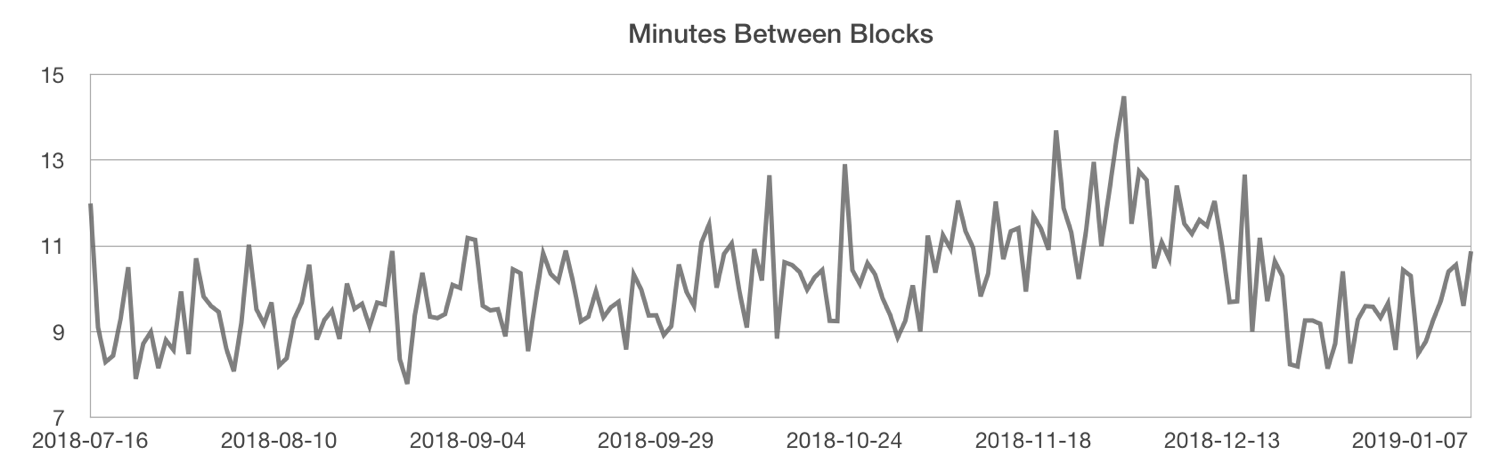
\includegraphics[width=\textwidth]{images/fig7.png}
    \caption{\footnotesize{\textit{De tijd tussen de blokken varieert, afhankelijk van de wisselende hash-snelheid en de factor toeval.}}}
    \label{fig7}
\end{figure}


\section{Moeilijkheidsaanpassing: consensus over het doelnummer}

Aangezien Bitcoin een vrijwillig en permissieloos systeem is waaraan mensen naar eigen inzicht kunnen deelnemen zonder dat er een centrale leiding is, zal het aantal miners in het netwerk sterk fluctueren. We moeten een manier vinden om de productie van blokken constant te houden, in plaats van dat er steeds versnellingen of vertragingen in de productie optreden wanneer miners zich toevoegen of zich terugtrekken.

Hoe kunnen we het lastiger maken om geldige hashes te vinden als er meer deelnemers zijn bij de loterij, en eenvoudiger als er deelnemers vertrekken? Op die manier zouden we de uitgifte en de intervallen tussen blokken stabiel kunnen houden.

Herinner je dat het minen van bitcoin een loterij is, waarbij je een willekeurig getal moet vinden dat kleiner is dan het doelnummer. Bitcoin lost dit probleem op door de moeilijkheidsgraad aan te passen. Aangezien iedereen dezelfde code uitvoert die dezelfde regels naleeft, en iedereen een volledige kopie heeft van de transactiegeschiedenis, kan iedereen onafhankelijk berekenen hoe snel blokken op dat moment worden geproduceerd.

\begin{figure}[h]
    \centering
    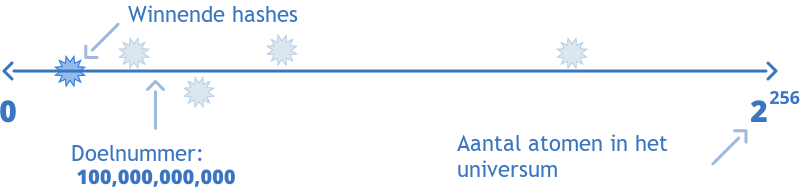
\includegraphics[width=\textwidth]{images/fig5.png}
    \caption{\footnotesize{\textit{We proberen dit kleine doel te bereiken. Het aantal mogelijke resultaten is onvoorstelbaar groot, dus het kan een eeuwigheid duren als we het proberen te bereiken door lukraak met de dobbelstenen te gooien.}}}
    \label{fig8}
\end{figure}

Elke keer wanneer we 2016 blokken hebben geproduceerd (dit duurt ongeveer 2 weken)\footnote{De aanpassingsperiode van 2016 blokken is op basis van het beoogde blokinterval van 10 minuten; 10 minuten x 2016 blokken = twee weken. Het blokinterval werd arbitrair vastgesteld door Satoshi om groot genoeg te zijn zodat de meeste nodes kunnen op de hoogte zijn van de laatste blok. De periode van twee weken is ook ietwat arbitrair gekozen, maar is ontworpen om te voorkomen dat het spel belazerd wordt door te snelle achtereenvolgende aanpassingen in de hash-rate.}, analyseren we de uitgiftesnelheid over die voorbije periode. We berekenen hoeveel tijd er nodig was om deze 2016 blokken te vervaardigen, en passen vervolgens het streefgetal aan om de productie van de blokken te versnellen of te vertragen.

Iedereen neemt de laatste 2016 blokken en deelt ze door de tijd die gemiddeld nodig was om te ze creëren. Was het gemiddelde meer dan 10 minuten? Dan gaan we te traag. Lag het gemiddelde onder de 10 minuten? Dan gaan we te snel.

We kunnen nu het streefgetal aanpassen, groter of kleiner maken, afhankelijk van hoe langzaam of snel we voortgaan, om ervoor te zorgen dat we in overeenstemming blijven met het afgesproken tijdsinterval van 10 minuten. Het doelgetal kan worden verhoogd, waardoor een breder scala aan hashes als geldige oplossing wordt beschouwd. Dit vergroot de kans voor miners om een winnende hash te vinden en vermindert de energie die ze nodig hebben om een blok te vinden. Dit wordt het verlagen van de moeilijkheidsgraad genoemd.

Aan de andere kant kunnen we het doelnummer kleiner maken, waardoor er minder hashes geldig zijn en miners meer energie moeten besteden aan het vinden van een blok. Dit noemen we het verhogen van de moeilijkheidsgraad. Dit houdt in dat we voor elke periode van 2016 blokken exact weten wat het richtgetal is. Dit biedt ons de magische grens waarbinnen een hash van het proof-of-work moet liggen om binnen die periode een winnend lot te verkrijgen.

\begin{figure}[h]
    \centering
    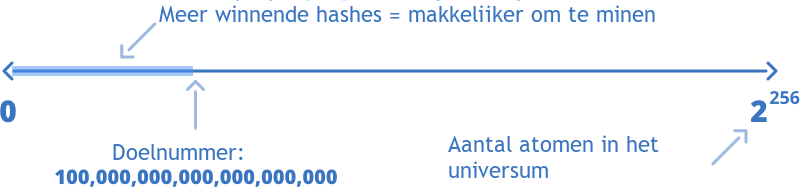
\includegraphics[width=\textwidth]{images/fig8.png}
    \caption{\footnotesize{\textit{Het verhogen van het doel vergroot de geldige ruimte, waardoor het waarschijnlijker wordt om in minder pogingen een juiste oplossing te vinden. Daardoor wordt het goedkoper in verbrande \mbox{energie.}}}}
    \label{fig9}
\end{figure}

Misschien zijn de aanpassingen van de moeilijkheidsgraad en het doelgetal wel de belangrijkste innovaties van Bitcoin. Deze maken het voor iedereen mogelijk om op een onafhankelijke manier de lotnummers te verifiëren. Deze lotnummers zijn op hun beurt weer gebaseerd op een doelgetal, dat ook onafhankelijk te verifiëren is. Zo kunnen we een soort loterij spelen zonder dat iemand ons de winnende combinatie moet onthullen.

In Figuur \ref{fig10} zie je de \textit{hash-rate} (lijn) en de moeilijkheidsgraad (staven) doorheen de tijd. De moeilijkheid wordt iedere 2016 blokken aangepast en lijkt een beetje op een trap. Telkens wanneer de hash-rate boven de moeilijkheid uitstijgt, zie je dat de moeilijkheidsgraad stijgt om bij te benen. Wanneer de hash-rate zakt, zoals tussen oktober en december 2018, zakt ook de moeilijkheidsgraad. De aanpassing van de moeilijkheidsgraad volgt altijd wat de hash-rate doet met een vertraging van 2016 blokken (twee weken).

\begin{figure}[h]
    \centering
    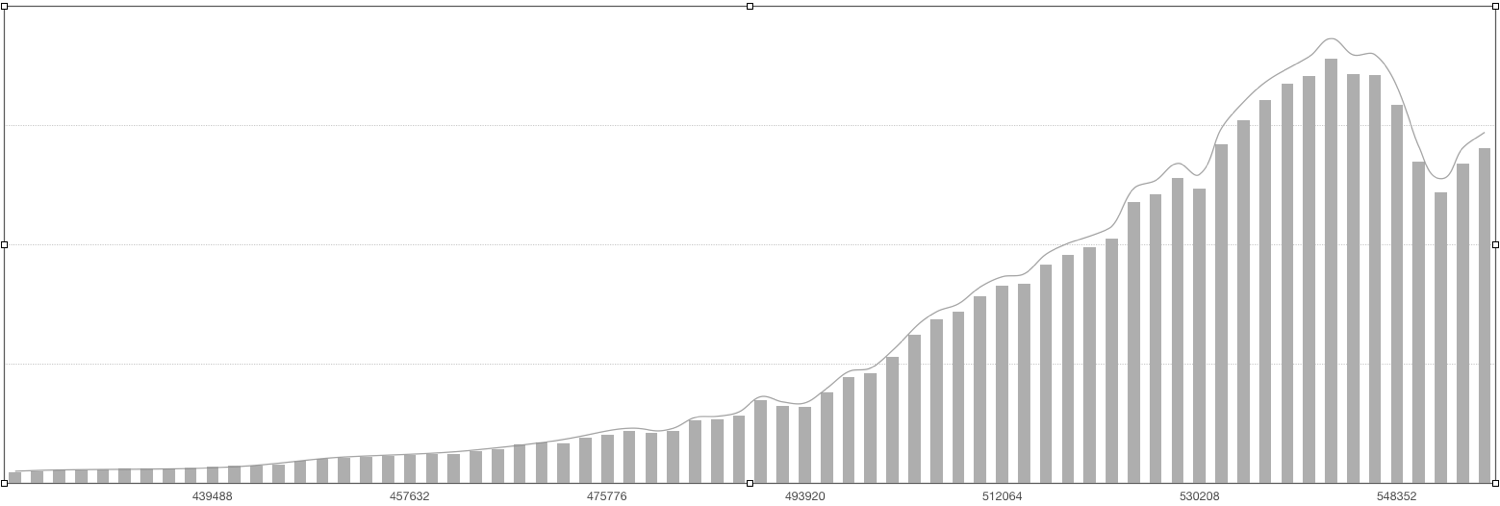
\includegraphics[width=\textwidth]{images/fig10.png}
    \caption{\footnotesize{\textit{Hash-snelheid versus moeilijkheid.}}}
    \label{fig10}
\end{figure}

Omdat er een vertraging van 2016 blokken zit in de aanpassing, kan het voorkomen dat aanzienlijke stijgingen of dalingen in de hash-snelheid resulteren in over- of onderproductie van bitcoins in die periode, waardoor er enigszins wordt afgeweken van het geplande uitgifteschema.

Het verhogen van de hash-snelheid gaat hand in hand met het produceren van veel nieuwe hardware. Hierdoor zijn pieken tamelijk ongebruikelijk en hebben ze niet al te veel invloed. De impact van elke piek, of deze nu stijgt of daalt, zal beperkt blijven tot dat interval van 2016 blokken. Na de volgende aanpassing keren we weer terug naar het gemiddelde van 10 minuten per blok.

\clearpage
\section{Hash-snelheid en de dollarwaarde van bitcoin}

Bitcoin past automatisch de moeilijkheidsgraad aan op basis van de totale rekenkracht van de deelnemers aan de ``loterij'', oftewel de miners die energie verbruiken om te hashen. Op deze manier wordt de fysieke wereld vervlochten met onze digitale wereld. De waarde van bitcoin, de kosten van hardware en energie en de complexiteit van het doelgetal creëren samen terugkoppelingsmechanismen.

\begin{enumerate}
\item Speculanten kopen bitcoin omdat ze denken dat de prijs hoger gaat, waardoor ze de prijs opdrijven tot \$X.
\item Miners verbruiken tot \$X aan energie en hardware om bitcoins te verdienen.
\item Een grote vraag van kopers duwt de prijs omhoog en leidt tot meer miners die aardig verdienen aan hun activiteit.
\item Meer miners betekent meer hash-rate en meer verbruikte energie om bitcoin te produceren. Het netwerk wordt nog sterker beveiligd. De kopers worden gerustgesteld door de veiligheid van het netwerk en drijven de prijs soms nog verder omhoog.
\item Na 2016 blokken gaat de moeilijkheidsgraad omhoog door de aanwezigheid van meer hash-rate.
\item Een hogere moeilijkheid betekent een lager doelnummer. De miners vinden nu minder vaak blokken waardoor sommigen meer dan \$X spenderen in kosten om een bitcoin te minen.
\item Voor sommige miners blijkt het niet meer interessant om te minen, omdat ze meer energie verbruiken dan de winst die hun activiteit oplevert wanneer ze hun bitcoin verkopen. Ze leggen hun machines af en de hash-rate op het netwerk gaat terug omlaag.
\item De volgende 2016 blokken passeren. De moeilijkheid wordt opnieuw berekend en aangezien sommige miners offline gingen, wordt het deze keer makkelijker. Het doelnummer gaat omhoog.
\item De lagere moeilijkheid betekent dat miners, die voorheen onrendabel waren, hun machines terug aanzetten of dat nieuwe miners op het toneel verschijnen.
\item Ga terug naar 1.
\end{enumerate}
In een neerwaartse markt kan de cyclus in de andere richting gaan. Gebruikers van het netwerk dumpen dan hun munten, de prijs gaat omlaag en miners worden onrendabel.

Het algoritme voor de aanpassing van de moeilijkheidsgraad zorgt dat er altijd een evenwicht wordt gevonden tussen de prijs en de hoeveelheid hash-rate die aanwezig is op het netwerk. Zelfs als de prijs drastisch zou zakken en de helft van de huidige hash-rate uit het netwerk zou duwen, dan zou de volgende aanpassing het opnieuw rendabel maken op een nieuw evenwichtsniveau.

De manier waarop de moeilijkheidsgraad wordt aangepast, zorgt ervoor dat inefficiënte miners plaats moeten maken voor degenen die werken met de goedkoopste mogelijke energie en de laagste totale operationele kosten. Na verloop van tijd stuurt dit bitcoin miners naar afgelegen plekken op de aarde. Ze gebruiken energiebronnen die onderbenut of helemaal niet benut zijn. Volgens een rapport van CoinShares uit 2019 maakt ongeveer 75\% van de bitcoin miners gebruik van hernieuwbare energiebronnen..\footnote{Lees meer over de laatste stand van zaken betreffende mining op \href{https://coinshares.com/research/bitcoin-mining-network-june-2019 }{https://coinshares.com/research/bitcoin-mining-network-june-2019 }}

De laatste jaren ging de prijs pijlsnel omhoog, net als de totale hash-rate. Hoe hoger de hash-rate, hoe moeilijker het is om het netwerk aan te vallen. Om te bepalen wat in het grootboek komt, moet je ten minste evenveel energie en hardware beheren als de helft van het hele netwerk. Op vandaag wordt geschat dat de elektriciteit die gebruikt wordt door bitcoin miners equivalent is met het verbruik van een land van gemiddelde grootte.

\section{Vergoedingen en het einde van blokbeloning}

Hoe kunnen we waarborgen dat miners nog steeds gemotiveerd blijven om energie te investeren in de beveiliging van het netwerk wanneer de blokbeloning uiteindelijk wegvalt? Het antwoord ligt in de transactiekosten. Na verloop van tijd nemen deze kosten de plaats in van de beloning en geven ze miners ook een stimulans om daadwerkelijk transacties in een blok te verwerken. Zonder deze prikkel zouden ze namelijk perfect in staat zijn om lege blokken te genereren en enkel de blokbeloning te incasseren.

De tarieven worden vastgesteld op een vrije markt waar gebruikers bieden op de gelimiteerde ruimte binnen een blok. Diegenen die transacties uitvoeren geven aan hoeveel vergoeding ze bereid zijn te betalen aan de miners. Op hun beurt hebben de miners de keuze om de transactie al dan niet op te nemen in het volgende blok, gebaseerd op die biedingen. Wanneer er slechts een beperkt aantal transacties in het volgende blok willen, zullen de vergoedingen laag zijn en is er minder concurrentie. Maar als de ruimte in de blokken schaars wordt, zullen gebruikers meer geneigd zijn om een hogere vergoeding te betalen om hun transactie sneller bevestigd te krijgen (in het volgende blok). Wie niet bereid is te betalen kan een lagere transactievergoeding instellen, maar moet dan wel rekening houden met een langere wachttijd.

In traditionele financiële systemen worden de kosten meestal berekend op basis van een percentage van het transactiebedrag. Bij Bitcoin maakt het echter niet uit hoeveel de overdracht waard is bij het berekenen van de vergoeding. In plaats daarvan worden de vergoedingen bepaald op basis van de schaarse grondstof die ze gebruiken, namelijk de ruimte in een blok. Deze kosten worden uitgedrukt in satoshi’s per byte van gebruikte blokruimte.\footnote{Een byte is 8 bits.} Het kan dus voorkomen dat een transactie van een miljoen bitcoins tussen twee partijen minder vergoeding kost dan een transactie waarbij 1 bitcoin wordt verdeeld over tien ontvangers, omdat deze laatste meer ruimte inneemt in de transactielijst.

Tijdens periodes waarin bitcoin enorm in trek was, zoals de grote stierenmarkt van 2017, gingen transactievergoedingen door het dak. Sindsdien zijn een aantal nieuwe functies geïmplementeerd die het probleem van hoge transactiekosten op het netwerk verlichten.

Een van die aanpassingen is \textquotedbl{}Segregated Witness\textquotedbl{}. Deze aanpassing zorgt voor een andere voorstelling van de data in blokken. Transacties die gebruik maken van die upgrade kunnen meer dan de originele 1MB aan blokruimte gebruiken (via een aantal slimme trucs die niet verder toegelicht worden in dit boek).

Nog iets dat bijdraagt aan het verlagen van de hoge transactiekosten is \textit{batching}. Grote handelsbeurzen en -platformen in het ecosysteem begonnen met het bundelen van transacties voor verschillende gebruikers in één: in tegenstelling tot traditionele betalingen via de bank of PayPal, die altijd geld van één persoon naar een andere sturen, kan een bitcointransactie een groot aantal inputs combineren en een groot aantal outputs produceren. Een beurs die bitcoin wil versturen om uit te betalen aan 100 verschillende gebruikers kan dat dus perfect doen in een enkele transactie. Op die manier wordt schaarse blokruimte veel efficiënter gebruikt. Wat ogenschijnlijk slechts enkele transacties per seconde zijn, kunnen in realiteit perfect duizenden transacties inhouden.

Met \textit{SegWit} en \textit{batching} komen we al een heel eind om de vraag naar blokruimte te verlagen. Verdere verbeteringen zullen het gebruik van blokruimte nog efficiënter maken. Niettemin zal er opnieuw een dag komen dat transactievergoedingen terug oplopen en blokken door de grote vraag naar blokruimte weer voller en voller raken.

We hebben nu bijna alle aspecten van bitcoin onder de loep genomen:

\begin{enumerate}
\item Centrale bank vervangen door een gedistribueerd grootboek.
\item Een loterij opgezet om te bepalen wie in het grootboek mag schrijven.
\item Spelers van de loterij worden verplicht om energie te gebruiken om lotjes te bemachtigen (door te hashen). Het is voor iedereen eenvoudig om een winnend lot te verifiëren door de hash naast ons eigen, onafhankelijk bepaald, doelnummer te leggen.
\item Duidelijke regels voor de deelnemers: wie de regels niet volgt, zal niet geaccepteerd worden. Hun blok met beloning in de zogenaamde \textit{coinbase}-transactie wordt dan verworpen en ze ontvangen geen bitcoin. Op die manier ontmoedigen we valsspelen en bieden we een economische stimulans om de regels te volgen.
\item Controle over de timing en selectie van het doelnummer voor de loterij door iedereen te laten berekenen wat het doelnummer moet zijn op basis van vastgelegde regels in de software en de geschiedenis van de laatste 2016 blokken.
\item Handhaven van het uitgifteschema door moeilijkheidsgraad aan te passen als gevolg van een hogere of lagere hash-rate.
\item Gebruik van \textit{open source} code om ervoor te zorgen dat iedereen voor zichzelf kan verifiëren dat zij dezelfde regels hanteerden betreffende geldigheid van transacties, blokbeloning en moeilijkheidsaanpassing.
\end{enumerate}
Geen centrale autoriteit meer. We hebben nu een volledig gedistribueerd en decentraal systeem. Dat is bijna het volledige plaatje. Eén probleem rest ons nog. Wanneer een nieuwe deelnemer aansluit bij het netwerk en een kopie van het grootboek opvraagt, kunnen ze van verschillende \textit{nodes} afwijkende geschiedenissen ontvangen. Hoe zorgen we voor een enkele, lineaire geschiedenis en hoe voorkomen we dat miners het verleden herschrijven?

